\section{Presentation Interface}
As first introduced in \cref{MDCI} the system should include a presentation interface. The concept of this interface is to avoid guests from accessing their devices, just to check the current playlist configuration, and instead provide quick and easily accessible overview for the guests of the system. By having a separated screen from the guests' devices, the system should reduce the amount of time guests spend using their devices, which was declared a problem best seen minimised, as concluded in \cref{sub:user_requirements}. The intention is to have the playlist on a screen above the bar, as visually envisioned in \cref{fig:PresentationInterface}. The screen should direct the guests' attention towards the bar, by making the playlist more accessible to the guest as the screen is bigger in size and always on, opposed to the small handheld device \cite{DEB}. It is important to stress that the screen should not be visually blockable by a person or other objects.

This is a part of the system which should always be visually accessible to the guest, therefore should also be visually pleasing to look at, but still contain all the information needed by the guest. An interesting problem to solve, is having to display each individual's votes in an efficient way, without providing an overflow of information, confusing the guest. One suggested solution is to have the most distinguishing content to the left with the reading direction, and the least distinguishing content to the right \cite{material}. In the presentation view, a track's placement on the playlist is placed on the left hand side and the amount of votes on the right hand side. Depicting individual guests will require some sort of ID, through a login or similar, to distinguish guests.

\begin{figure}[hbtp]
  \centering
  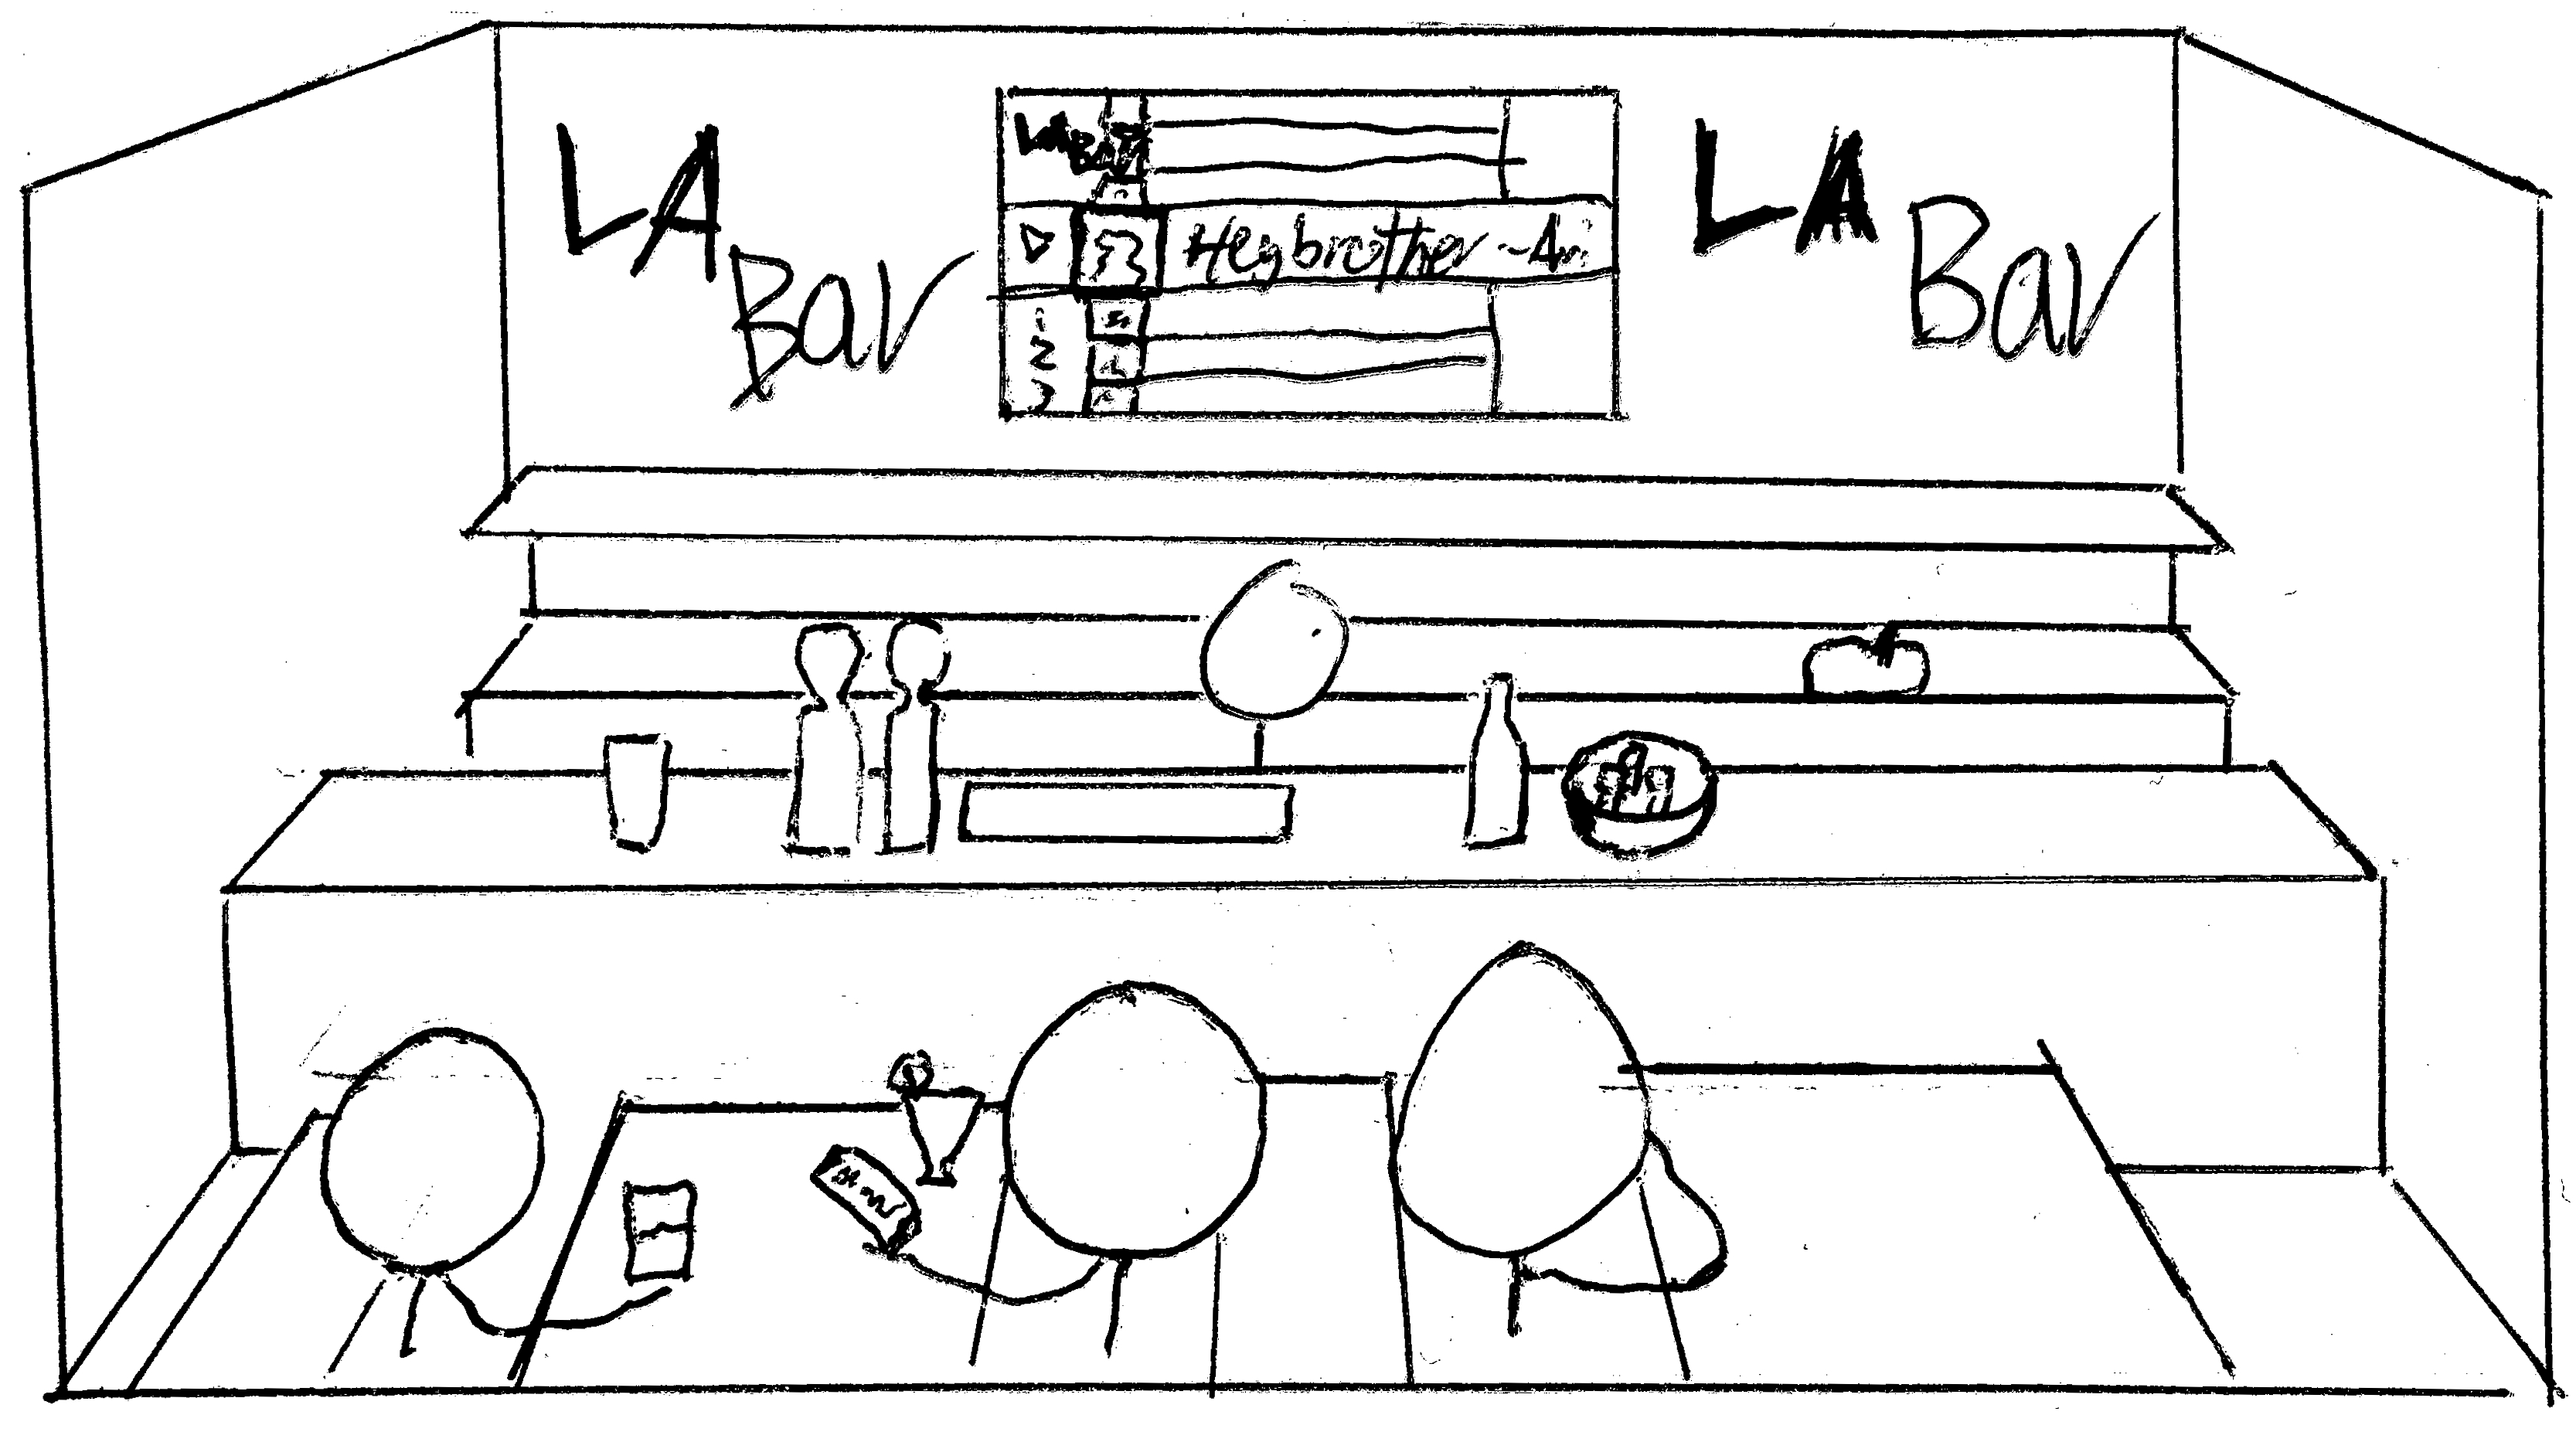
\includegraphics[width=1.0\linewidth]{Images/presentation.png}
  \caption{Sketch of the screen in context and visual design.}\label{fig:PresentationInterface}
\end{figure}

\begin{figure}[hbtp]
  \centering
  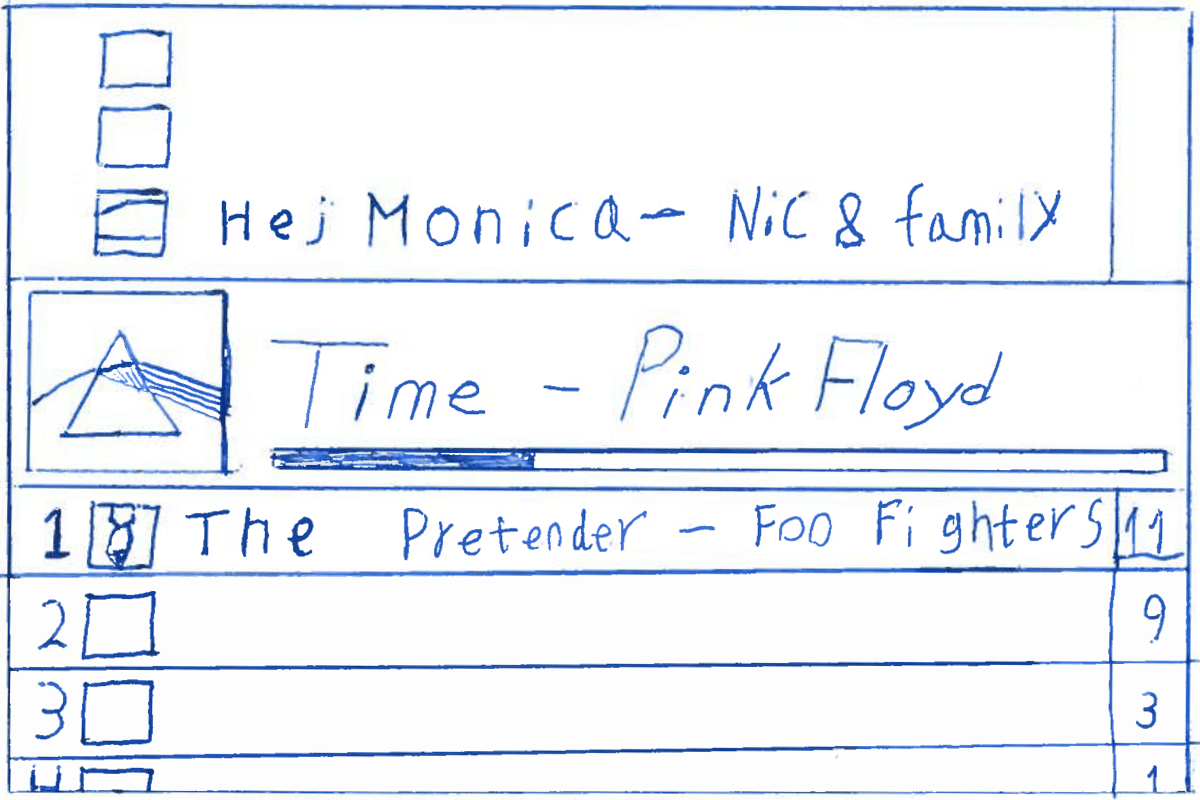
\includegraphics[width=1.0\linewidth]{Images/presentationInterface.png}
  \caption{A sketch of the visual design of the presentation interface.}\label{fig:presentation}
\end{figure}

The presentation view is designed to show the current playing track, the history and the tracks to be played next, according to the current votes. The currently playing track will be shown in the vertical middle of the screen. The history will be displayed above as a list of tracks, ordered with the last played track at the bottom. Below the current playing track a list of tracks will display the tracks guests have voted on. The highest voted track will be in the top of the list as shown on figure \cref{fig:presentation}. 

%Sørensen and Kjeldskov did an article on interaction with a similar system. They found some field test 
